\documentclass[a4paper,11pt]{article}

\usepackage{amsmath}
\usepackage{amsfonts}
\usepackage{dirtytalk}
\usepackage{physics}
\usepackage{biblatex}
\usepackage{hyperref}
\usepackage{refcheck}
\usepackage{booktabs}
\usepackage{multirow}
\usepackage{longtable}
\usepackage{float}
\usepackage[font=normalsize]{caption}
\usepackage{graphicx}
\setkeys{Gin}{width=.8\textwidth}
\graphicspath{ {./images/} }
\usepackage{indentfirst}
\addbibresource{ref.bib}


\font\Bbb=msbm10 at 11pt
\def\QQ{\mbox{\Bbb Q}}
\def\RR{\mbox{\Bbb R}}
\def\ZZ{\mbox{\Bbb Z}}
\def\NP{{\cal NP}}

\newtheorem{definition}{Definition}
\newtheorem{lemma}{Lemma}
\newtheorem{proposition}{Proposition}
\newtheorem{remark}{Remark}
\newtheorem{theorem}{Theorem}


\newenvironment{proof}
{\begin{trivlist} \item[] {\bf Proof.\ }}{\hfill$\Box$ \end{trivlist}}

\title{Using Sensitivity Analysis from Stochastic Programs to Inform Marketing Decisions}

\author{Congzheng Liu\thanks{Department of Management Science,
Lancaster University, Lancaster LA1 4YX, UK.
Email: {\tt \{c.liu19,a.n.letchford,i.svetunkov\}@lancaster.ac.uk}}
\and Adam N.\ Letchford$^*$ \and Ivan Svetunkov$^*$} % end author list

\date{8th July 2020}

\begin{document}

\maketitle

\begin{abstract}
Inventory control has always been crucial in Operations Research and Operations Management. It is particular important for companies to update their decisions in the dynamic marketing environment. 
We formulate a single-period multi-product Newsvendor problem (MPNP). We then show how one can use sensitivity analysis to inform marketing decisions. In particular, we can estimate the marginal increase/decrease in
costs that one could expect from new information.
\\*[2mm]
{\bf Keywords:} newsvendor problems; stochastic programming; inventory control; sensitivity analysis
\end{abstract}

\section{Introduction}
Inventory control has always been treated as an important part of Operations Research and Operations Management \cite{Po02,SPP98,Zi00}. In this paper, we consider a production planning problem, which can be viewed as a kind of single-period multi-product
Newsvendor problem (MPNP)\cite{D98,TTV12}.

In general, MPNP considers the manufacturing and/or retailing procedure in a company with multiple products \cite{SPP98}. Regarding to the natures of applier, the constraints in MPNP could be manufacturing abilities, storage capacities or funding powers, etc. Here, we refer as resources for convenience. In this paper, we assume the applier is a factory, and we use manufacturing terms in formulation. In this case, the goal of MPNP is to decide the optimal quantities of each product to be manufactured regarding to a given cost function, while satisfies all dimensions of resource at the same time \cite{BDR12}. The cost function is similar to the classical Newsvendor problem \cite{Ch12}, where the expected cost is formed by \emph{over-stocking cost}, \emph{under-stocking cost} and stochastic demand.

In practice, demand of products are estimated by experts in field of forecasting. The quantities deciding process, however, is an optimisation problem, which can be handled by computational experts. This two stage method is usually called disjoint method, in contrast with integrated method, which usually derive decision directly from data \cite{Sc58}. 

In this paper, we concentrate on the second stage of the disjoint method. Specifically, we focus on post-optimisation phase where \emph{new information} alters our decision, which is referred as 'sensitivity analysis' in field of optimisation \cite{D98,Ga03,Va20}. We use linear program (LP) with generated scenario set to approximates the stochastic feature of MPNP, and use the reduced cost/shadow price to inform marketing decision. This method is stable and very efficient. We don't need to resolve the optimisation problem, but apply our sensitivity analysis results as long as the changes in allowable interval.

The rest of this paper is organized as follows. Section \ref{se:lit} presents works in previous literature. Section \ref{se:model} specificates the model. Section \ref{se:sensitivity} contains the sensitivity analysis with an example. Section \ref{se:extensions} presents extensions to the analysis.
%%%%%%%%%%%%%%%%%%%%%%%%%%%%%%%%%%
\section{Literature Review}
\label{se:lit}
MPNP is one extension of classical Newsvendor problem (NVP). Here we assume readers are familiar with the basic of NVP. The reader looking for more background knowledge is directed to the books \cite{Ch12,Po02,SPP98}.

\subsection{Multi-product Newsvendor problem}
\label{sub:lit_mpnp}
In the traditional MPNP, found in \cite{HW63,NS84}, a manufacturing company is interested in determining quantity $x_j$ for product $j (j=1,\dots,n)$ to satisfy the demand. For each product, the demand is assumed to be stochastic, defining as ${\tilde d}_j$ with known distribution (could also be partial distribution). Yet, products left over are punished with $c_j^o$ per unit, while shortfall are punished with $c_j^u$ per unit. For a risk neutral manufacturer, the goal is then:

\begin{equation}
    \min \quad \sum_{j=1}^n \mathop{\mathbb{E}} \big( c^o_j \big[  x_j - {\tilde d}_j \big]^+ \, + \, c^u_j \big[ {\tilde d}_j - x_j \big]^+ \big).
\label{eq:uncon}
\end{equation}

It follows that the first order conditions (FOCs) for optimizing (\ref{eq:uncon}) are
necessary and sufficient to determine the optimal quantity of $x_j$. Based on this, we have:
\[
    x_j^* = F_j^{-1}\left( \frac{c_j^u}{c_j^o+c_j^u} \right),
\]
where $F_j$ is the underlying cumulative distribution function for ${\tilde d}_j$.

In practice, one could add constraints to the optimisation. In general, we set:
\[
    \sum_{j=1}^n s_{ij} x_j \le S_i	\quad (i = 1, \ldots, m),
\]
where $s_{ij}$ denotes the resource required per unit of product $j$ in dimension $i$, and $S_i$ denotes the maximum capacity of resource dimension $i$.

When the resource is one-dimension, it has been studied that one can use a Lagrange multiplier technique to find the optimal order quantity in this setting \cite{HW63}. This technique is straightforward and efficient. Yet, in some practical situations, the optimal $x_j$ will tend to be very small and using this technique could lead to deviations. Other approaches for one-dimension constraint MPNP are available in \cite{ALM05,NS84,ZXH09,Zh10}.

For multi-dimension constraint MPNP, MPNP with substitution and other extensions, readers can find reference in \cite{BAA99,BR93,CVW14,LL95,MS78}. 

\subsection{Stochastic linear programming}
%\label{sub:lit_sto}
Given the nature of underlying uncertainty, one approach to approximate MPNP is stochastic programming \cite{Bea55,D98}. Specifically, we would introduce the two-stage stochastic linear programming with recourse (stochastic LP), which is built from a collection of multi-period linear programs, each having the same structure but somewhat different data. See book \cite{HS13,KM76,KWK94,Pf12} for reference. A general stochastic LPs with $K$ scenarios may be regarded as having the following form:
\begin{eqnarray}
\label{eq:sto_obj}
    \min	& f ( u ) + \sum_{k \in K} g^k ( v^k )\\
\label{eq:sto_cons1}
	\text{s.t.}    & V_0 u \leq p\\
\label{eq:sto_cons2}
	& V_k u +W_k v^k \leq q^k\\
\label{eq:sto_posi}
	& u, v^k \geq 0.
\end{eqnarray}
where $f$ and $g$ are linear cost functions, $V$, $W$, $p$ and $q$ are parameters. The vectors $u$ contains the first-stage variables, whose values must be chosen immediately, while the vector $v$ contains all of the variables for subsequent periods. The constraint (\ref{eq:sto_cons1}) involves only first-stage variables and are the same in every scenario, and constraints in (\ref{eq:sto_cons2}) involve variables of second-stage and differ in some respects from scenario to scenario, reflecting uncertainty about the future.

With a finite number of scenarios, this stochastic LP can be viewed as large linear programming model \cite{KW12}. Thus, one can perform sensitivity analysis on the model \cite{AW93,Du95}.

\subsection{Sensitivity Analysis}
%\label{sub:lit_sen}
The term sensitivity analysis has been used widely. Readers can find applications in books \cite{KCH86,SRA08,STCR04}. In this paper, we consider especially the sensitivity analysis within LP. According to textbook definitions \cite{DT06}, we first transfer the model into standard form:
\begin{eqnarray*}
    \min	& b^T x = h \\
	\text{s.t.}    & A \, x = p\\
	& x \geq 0,
\end{eqnarray*}
where $x \in \RR_+^n$ denotes the variable vector including slack variables, $\pi \in \RR_+^m$ denotes the dual vector, and $A: m \times n$ is the coefficient matrix. We also have its dual:
\begin{eqnarray*}
    \max	& p^T \pi = r \\
	\text{s.t.}    & A^T \pi \leq b.
\end{eqnarray*}
Let $x^*$ be the optimal primal
solution, and let $\pi^*$ be the corresponding dual solution. It is shown by strong duality \cite{BGW09,DT06}:
\[
    h^* = b^T x^* = p^T \pi^* = r^*
\]
Thus, we have $\pi_i^* = \pdv{h^*}{p_i}$ that is referred to as the \emph{shadow price} of $p_i$, and $\bar{b} = b - A^T \pi^*$ that is referred to as the \emph{reduced cost} vector. Given changes lying in allowable range, one can use those values to inform decisions. Derivation can be found in \cite{D98,DT06}.
%%%%%%%%%%%%%%%%%%%%%%%%%%%%%%%%%%
\section{Model Specification}
\label{se:model}
We consider following model. A company manufactures $n$ products on $m$ machines. Producing one unit of product $j$
takes $t_{ij}$ units of time on machine $i$. Machine $i$ can be used for at most $T_i$ time units. The demand of
product $j$ is a random variable ${\tilde d}_j$ with known distribution. Each unit of product $j$ produced in excess
of demand incurs an \emph{over-stocking cost} $c^o_j$. Each unit by which demand is unsatisfied incurs an
\emph{under-stocking cost} $c^u_j$. The company wishes to decide how much of each product to produce, in order
to minimise expected costs $C$. For simplicity, we permit fractions of products to be produced.

\subsection{Problem formulation}
%\label{sub:problem}
We formulate the problem as follows. For $j = 1, \ldots, n$, let $x_j$ represent the amount of product $j$ produced, then we wish to solve the following stochastic program (SP):

\begin{eqnarray*}
    \min & \sum_{j=1}^n \mathop{\mathbb{E}} \big( c^o_j \big[  x_j - {\tilde d}_j \big]^+ \, + \, c^u_j \big[ {\tilde d}_j - x_j \big]^+ \big) \\
	\text{s.t.}    & \sum_{j=1}^n t_{ij} x_j \le T_i	& (i = 1, \ldots, m) \\
	& x \in \RR_+^n.
\end{eqnarray*}

Following the standard approach \cite{BL11}, we can construct a stochastic LP that approximates the SP. Consider a set $S$ of
scenarios, i.e., realisations of demand obtained from marketing experience. We let $d_j^s$ denote the demand for product $j$ in scenario $s$. We also let $y_j^s$ be the number of units over-stocked (if any), and let $z_j^s$ be the number of units under-stocked (if any), respectively, in scenario $s$. The LP is then:
\begin{eqnarray}
\label{eq:obj}
    \min	& \sum_{s \in S} \sum_{j=1}^n \big( c^o_j y_j^s + c^u_j z_j^s \big) \\
\label{eq:time}
	\text{s.t.}    & \sum_{j=1}^n t_{ij} x_j \le T_i	& (i = 1, \ldots, m) \\
\label{eq:over}
	& y_j^s \ge x_j - d_j^s			& (s \in S; \, j = 1, \ldots, n) \\
\label{eq:under}
	& z_j^s \ge d_j^s - x_j			& (s \in S; \, j = 1, \ldots, n) \\
\label{eq:posi1}
	& x \in \RR_+^n				& \\
\label{eq:posi2}
	& y^s, z^s \in \RR_+^n			& (s \in S).
\end{eqnarray}

Denote the solution of SP to be $x^*$ and the solution of LP to be $x_L^*$. It has been studied that $x_L^*$ converges to $x^*$ as $|S| \to \infty$. References are available in \cite{G00,KR93,R96}.

\subsection{Information Formulation}
\label{sub:information}
Two sources of new information are concentrated: 1). \emph{Retailing effort} that alter the mean/variance of demand deliberately. 2). \emph{Manufacturing effort} that loosen/tighten manufacturing constraints or increase/decrease costs. Readers can apply same technique on other sources of new information intuitively.

We formulate margin of the information mathematically.

Consider there exists particular retailing effort that could manually alter the mean demand of a single product $j'$. If the mean demand increased by some quantity $\bar{\epsilon}$, then the right-hand sides of the corresponding constraints (\ref{eq:over}) and (\ref{eq:under}) would increase by $\bar{\epsilon}$. If we denotes $S_{\bar{\epsilon}}$ to be the set of all scenarios whose constraint is influenced by $\bar{\epsilon}$, the margin can be expressed as:
\[
    \Delta \, C_{\bar{\epsilon}} = \sum_{s \in S_{\bar{\epsilon}}} \pi_s^* \bar{\epsilon}.
\]

Now suppose instead that there is a change in  variance. Let $\mu_j$ denote the mean demand for product $j$. To simulate a decrease in standard deviation of demand for product $j$ by $k\%$, we can alter each $d_j^s$ to $\mu_j + (1-\frac{k}{100}) \big( d_j^s - \mu_j \big)$. Accordingly, we should have an equivalence:
\[
\begin{aligned}
    \epsilon^s 
    & = \mu_j + (1-\frac{k}{100}) \big( d_j^s - \mu_j \big) - d_j^s\\
    & = \frac{k}{100} \big( \mu_j - d_j^s \big).
\end{aligned}
\]
Again, we can use shadow price to express the margin:
\[
    \Delta \, C_{k} = \sum_{s \in S_k} \pi_s^* \epsilon^s.
\]


Moreover, we consider manufacturing effort that update the manufacturing constraints. Suppose machine $i$ is wearing gradually, and it can only be used for at most $T_i + \Delta T_i$ time units now, where $\Delta T_i \leq 0$. We consider the simplest case, where the change only happens to single machine $i'$. The corresponding constraint (\ref{eq:time}) becomes:
\begin{eqnarray*}
    \sum_{j=1}^n t_{ij} x_j \le T_i + \Delta T_i	& (i = i').
\end{eqnarray*}
And the margin can be, again, calculated easily by product of the change of RHS and corresponding shadow price.

Besides the updating of machine capacity, It is also possible that a breakthrough of technology makes a particular product $j$ easier to recycle than before. Let's say, the over-stocking cost for product $j$ is now reduced to $c_j^o + \Delta c_j^o$, where $\Delta c_j^o \leq 0$. Again, we consider the simplest case where only one product $j'$ is affected. The objective (\ref{eq:obj}) becomes:
\begin{eqnarray*}
    \min \quad \sum_{s \in S} \big[ \sum_{j = 1}^n \big( c^o_j y_j^s + c^u_j z_j^s \big) + \Delta c_{j'}^o y_{j'}^s \big].
\end{eqnarray*}
Providing the changes in allowable range, the margin is $\sum_{s \in S} \Delta c_{j'}^o y_{j'}^s$.

\section{Sensitivity Analysis: An Example}
\label{se:sensitivity}

We now compute the shadow price, reduced cost, as well as the allowable range with an example. Then we consider the marginal increase/decrease in costs from new information.

\begin{table}[h]
\caption{Demand Realisations: Example}
\label{tab:demand}
\centering
\resizebox{\linewidth}{!}{
\begin{tabular}{ccccccccccccc}
\toprule
\multicolumn{1}{c}{\textbf{Products}} & \multicolumn{12}{c}{\textbf{Demand Realisations}} \\
\cmidrule(l{3pt}r{3pt}){1-1} \cmidrule(l{3pt}r{3pt}){2-13}
& $s_1$ & $s_2$ & $s_3$ & $s_4$ & $s_5$ & $s_6$ & $s_7$ & $s_8$ & $s_9$ & $s_{10}$ & $s_{11}$ & $s_{12}$\\
\midrule
product $a$ & 200 & 220 & 180 & 190 & 190 & 210 & 240 & 250 & 200 & 190 & 210 & 240\\
product $b$ & 250 & 230 & 200 & 180 & 210 & 210 & 170 & 150 & 180 & 220 & 260 & 260\\
\bottomrule
\end{tabular}}
\end{table}

\begin{table}[h]
\caption{Demand Realisations: Statistical Summary}
\label{tab:summary}
\centering
\resizebox{0.55\linewidth}{!}{
\begin{tabular}{ccc}
\toprule
 & product $a$ & product $b$\\
\midrule
mean & 210 & 210\\
standard deviation & 22.96 & 35.93\\
median & 205 & 210\\
1st quantile & 190 & 180\\
3rd quantile & 225 & 235\\
\bottomrule
\end{tabular}}
\end{table}

Suppose we manufacture 2 products on 3 machines. Producing one unit of product $a$ requires 4, 7 ,8 units of time on machine $A$, $B$ and $C$, respectively; Producing one unit of product $b$ requires 6, 5, 8 units of time on machine $A$, $B$ and $C$. The capacities of 3 machines are 2200, 2500 and 3500. Over-stocking cost for product $a$ and $b$ are 5 and 7, while under-stocking cost for product $a$ and $b$ are both 6. For demonstration, we only simulate 12 scenarios for demand. Data and statistics are presented in Table \ref{tab:demand} and \ref{tab:summary}.

There are 50 variables in total, $\big\{ x_1,x_2 \big\} \cap \big\{ y_1^1,\dots,y_1^{12},y_2^1,\dots,y_2^{12} \big\} \cap \big\{ z_1^1,\dots,z_1^{12},z_2^1,\dots,z_2^{12} \big\}$, and for each constraint, we assign a slack variable and/or an artificial variable. The problem can be solve easily with linear solver, with optimal $C=3437.14$, $x_1=207.1$, $x_2=210$. Full results see Table \ref{tab:sen_var} and Table \ref{tab:sen_con} in Appendix \ref{se:report}.

Now we consider the information described in \ref{sub:information}.

Suppose the mean demand of product $a$ or $b$ has been increased by $\bar{\epsilon}$. Regarding the 100\% rule \cite{BHM77}, we have:

\[
\begin{aligned}
    \Delta \, C_{\bar{\epsilon}_a} = 
    \begin{cases}
        6 \, \bar{\epsilon}_a, & \bar{\epsilon}_a \geq -2.88,\\
        unpredictable, & \text{otherwise}.
    \end{cases}\\
    \Delta \, C_{\bar{\epsilon}_b} = 
    \begin{cases}
        4.29 \, \bar{\epsilon}_b, & \bar{\epsilon}_b \geq -4,\\
        unpredictable, & \text{otherwise}.
    \end{cases}
\end{aligned}
\]

Similarly, if we consider a change of standard deviation on product $a$ or $b$, say, decreasing by $k\%$, we should have:
\[
\begin{aligned}
    \Delta \, C_{k_a} = -12.1 \, k_a,\\
    \Delta \, C_{k_b} = -22.1 \, k_b,
\end{aligned}
\]
providing the demand remain positive and variance is no less than zero.

One can compare these results with simulation outputs in Figure \ref{fig:mean} and Figure \ref{fig:var} for verification.
\begin{figure}[ht]
\centering
\caption{Optimal cost vs. Change of mean}
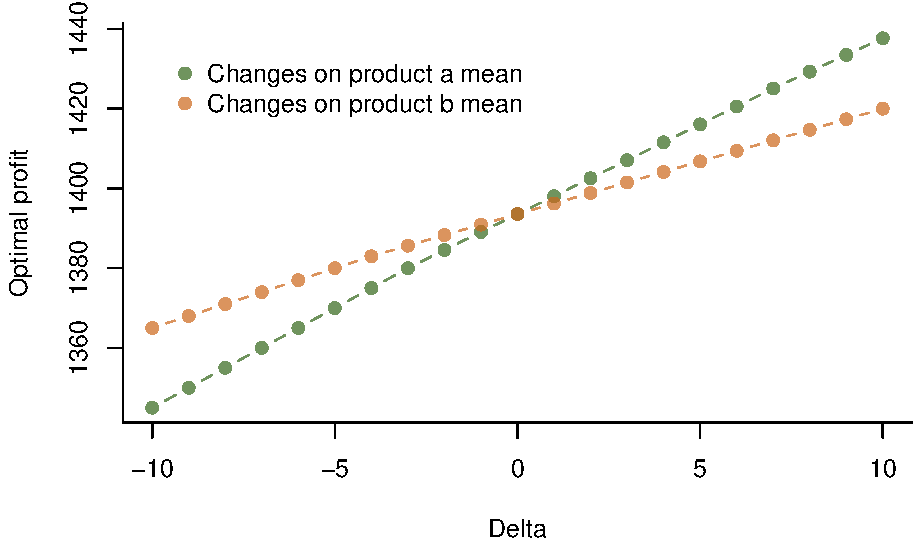
\includegraphics{Example-figure_files/figure-latex/mean-1.pdf}
\label{fig:mean}
\end{figure}

\begin{figure}[ht]
\centering
\caption{Optimal cost vs. Change of variance}
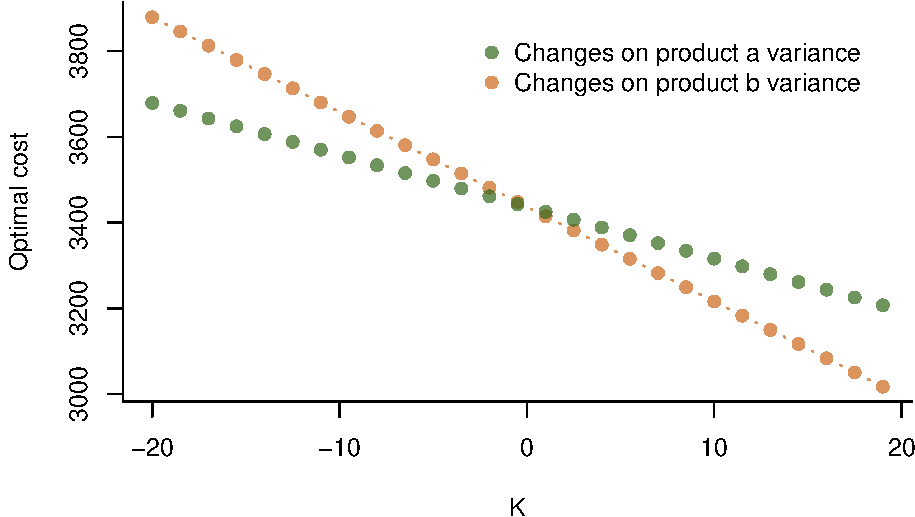
\includegraphics{Example-figure_files/figure-latex/var-1.pdf}
\label{fig:var}
\end{figure}

On the other hand, we could consider the manufacturing effort that works on constraint (\ref{eq:time}). We suppose machine $B$ is now going through maintenance, and can only be used for at most $T_B + \Delta T_B$ units of time. Given the fact time constraint on machine $B$ is binding, changes in will affect the cost. Thus:
\[
    \Delta \, C_{T_B} = 
    \begin{cases}
        -0.86 \, \Delta T_B, & -50 \leq \Delta T_B \leq 20,\\
        unpredictable, & \text{otherwise}.
    \end{cases}
\]
Yet, the time constraint on machine $A$ and machine $C$ is non-binding, changes in allowable interval will not affect the solution nor the cost.

Furthermore, we can consider the influence of altering variable coefficient. For instance, we consider there exists a technology breakthrough that reduces the over-stocking cost by recycling. Therefore:
\[
\begin{aligned}
    \Delta \, C_{c_a^o} = 
    \begin{cases}
        92.6 \, \Delta c_a^o, & -0.63 \leq \Delta c_a^o \leq 1,\\
        unpredictable, & \text{otherwise}.
    \end{cases}\\
    \Delta \, C_{c_b^o} = 
    \begin{cases}
        170 \, \Delta c_b^o, & -0.71 \leq \Delta c_b^o \leq 0.54,\\
        unpredictable, & \text{otherwise}.
    \end{cases}\\
\end{aligned}
\]
Simulation outputs see Figure \ref{fig:over}.

\begin{figure}[ht]
\centering
\caption{Optimal cost vs. Change of over-stocking cost}
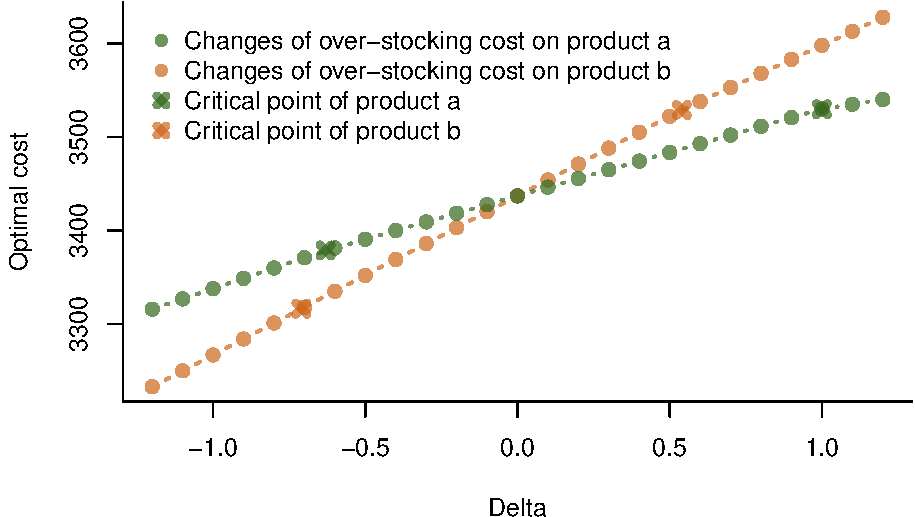
\includegraphics{Example-figure_files/figure-latex/c_o-1.pdf}
\label{fig:over}
\end{figure}

\section{Extensions}
\label{se:extensions}

We consider more complicated information intakes now, where two or more correlated parameters are changed simultaneously.

\subsection{Price-Demand Correlation}
%\label{sub:p-d}
Regarding the retailing effort we presented in \ref{sub:information}. The mean of demand can be deliberately increased by some amount $\bar{\epsilon}$, while all other parameters are fix. Yet, in practice, increase of demand is usually a trade-off by scarifying unit profit. From the formulation used in this paper, we consider the trade-off between mean demand and under-stocking cost. Readers can find reference in \cite{Ch12,Po02,SPP98} that provides explanation of viewing profit as opportunity cost.

Suppose we have linear price-demand correlation:

\[
    \mu_j = \alpha + \beta c_j^u,
\]
where $\alpha > 0, \beta < 0$ are parameters. Change of under-stocking cost on product $j'$ by $\Delta c_{j'}^u$ will now affect (\ref{eq:obj}), (\ref{eq:over}) and (\ref{eq:under}). The LP becomes:

\begin{eqnarray*}
    \min & \sum_{s \in S} \big[ \sum_{j = 1}^n \big( c^o_j y_j^s + c^u_j z_j^s \big) + \Delta c_{j'}^u z_{j'}^s \big]\\
    \text{s.t.}    & \sum_{j=1}^n t_{ij} x_j \le T_i	& (i = 1, \ldots, m) \\
	& y_j^s \ge x_j - d_j^s			& (s \in S; \, j \neq j') \\
	& y_{j'}^s \ge x_{j'} - d_{j'}^s - \beta \Delta c_{j'}^u           & (s \in S)\\
	& z_j^s \ge d_j^s - x_j			& (s \in S; \, j \neq j') \\
	& z_{j'}^s \ge d_{j'}^s + \beta \Delta c_{j'}^u - x_{j'}        & (s \in S)\\ 
	& x \in \RR_+^n				& \\
	& y^s, z^s \in \RR_+^n			& (s \in S).
\end{eqnarray*}
Furthermore, we can denotes $N^o$ as the number of scenarios that incur over-stocking and $N^u$ as the number of scenarios that incur under-stocking.

It has been shown very difficult to deal with joint perturbations on both objective function coefficient and constraint RHS mathematically. Thus, here we only consider the margin of changes while assuming any small changes we proposed are in the allowable range. 

To visualise our procedure, we consider again the two products example in Section \ref{se:sensitivity}, with $\alpha = 270, \beta = -10$. Higher dimension problem can be solve with same procedure, accordingly. Recalling the results from \ref{sub:lit_mpnp}, we can visualise the objective function as an oblique circular cone opening to the top with no boundary, while the feasible region is a convex polygon. See 3D plot in Figure \ref{fig:3d} and contour plot in Figure \ref{fig:con}.

\begin{figure}[ht]
\centering
\caption{3D plot of costs on two products}
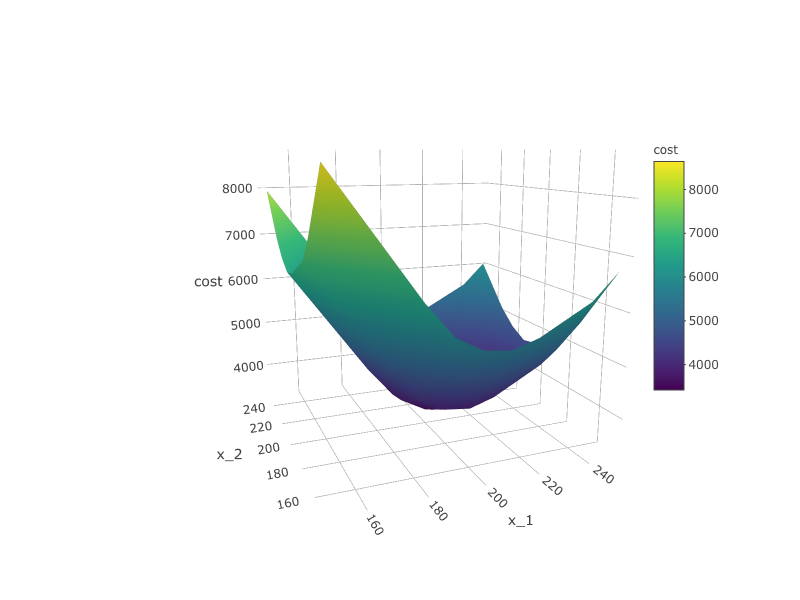
\includegraphics[width=0.9\textwidth]{Example-figure_files/figure-latex/3d cost.png}
\label{fig:3d}
\end{figure}

\begin{figure}[ht]
\centering
\caption{Contour of costs with boundaries}
\hspace{0.7cm}
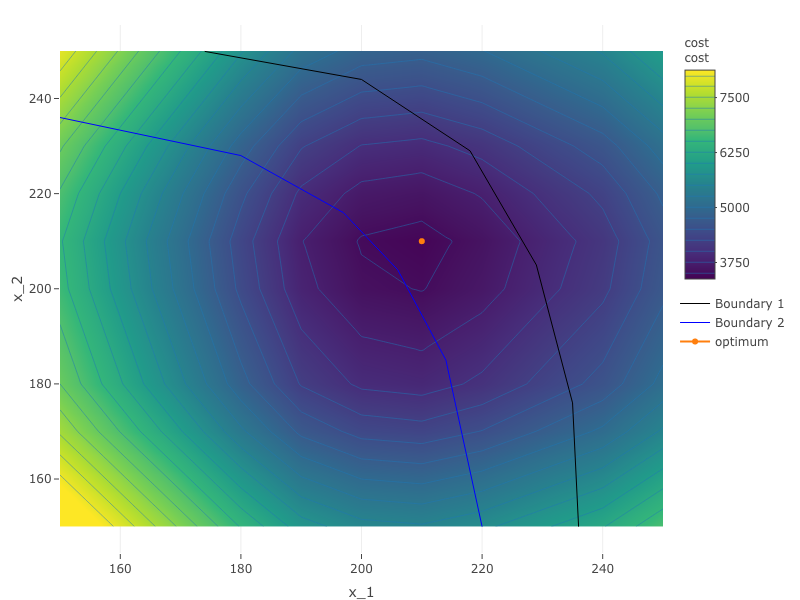
\includegraphics[width=0.9\textwidth]{Example-figure_files/figure-latex/contour.png}
\label{fig:con}
\end{figure}

In Figure \ref{fig:con}, we also include two example boundaries to demonstrate different kinds of feasible region (on the left side of boundary). Moreover, we define a \emph{prime point} to denote the optimal solution when all constraints are relaxed. One can see that boundary 1 forms a feasible region contains the prime point, while the feasible region formed by boundary 2 doesn't. There is no doubt that the optimal solution for MPNP with boundary 1 is lying exactly at the prime point, and the solution will remains optimal as long as the prime point is not 'pushed out' of the feasible region. On the other hand, one can easily show the optimal solution for MPNP with boundary 2 lies on the boundary since the cost function is convex \cite{DT06}, and the solution on this case is more sensitive. Costs on boundaries see Figure \ref{fig:bd1} and Figure \ref{fig:bd2} in Appendix \ref{se:costfun}.

Now, we consider the boundary for the example in Section \ref{se:sensitivity}. We have equation set:
\[
\begin{cases}
    4 x_1 + 6 x_2 \leq 2200\\
    7 x_1 + 5 x_2 \leq 2500\\
    8 x_1 + 8 x_2 \leq 3500,
\end{cases}
\]
that forms the boundary in Figure \ref{fig:conexam}. It is clear this feasible region doesn't include the prime point. Therefore, the optimal solution should lies on boundary, as we computed in Section \ref{se:sensitivity}. One can compare the relaxed solution, the prime point $\big( 210,210 \big)$, with the true optimal solution on boundary $\big( 207.1,210 \big)$.

\begin{figure}[ht]
\caption{Contour of cost with example boundary}
\hspace{1cm}
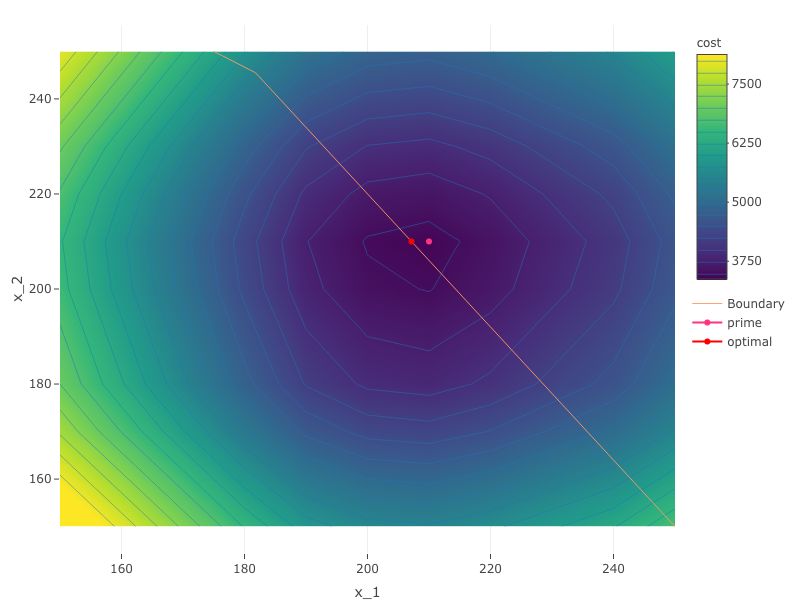
\includegraphics[width=0.9\textwidth]{Example-figure_files/figure-latex/conexam.png}
\label{fig:conexam}
\end{figure}

Moreover, we can visualise the effect on changes using contour plot. Any changes on demand will lead to the move of prime point, and any changes on costs will lead to the change on the density of contour lines. For instance, if we apply the price-demand correlation, and decrease the under-stocking cost of product $a$ by 0.6, the prime point will moves to the right by $|0.6\,\beta|$, along with all contour lines, and the contour lines at the left side of prime point will become looser. See new contour plot in Figure.


\subsubsection*{Margin of changes: Case 1}
We first consider the case where $x_j^*(j \neq j')$ and $y^*,z^*$ remain still, any changes on $\tilde{d}_{j'}$ are immediately absorbed by the changes on $x_{j'}$. We can derive easily:
\[
    \Delta \, C_{y^*z^*} = \Delta c_{j'}^u z_{j'}^s,
\]
and the new solution:
\[
\big( x_1^*,\dots,x_{j'}^*+\beta \Delta c_{j'}^u,\dots,x_n^*  \big)
\]

\subsubsection*{Margin of changes: Case 2}
For the case $x^*$, $N^o$ and $N^u$ remain still, changes on demand will directly lead to over-stocking/under-stocking.

We first define:
\[
    \Delta y_j^s =
    \begin{cases}
        -\Delta \mu_j, & y_j^s > 0,\\
        0, & y_j^s = 0,
    \end{cases}
\]
and,
\[
    \Delta z_j^s =
    \begin{cases}
        \Delta \mu_j, & z_j^s > 0,\\
        0, & z_j^s = 0.
    \end{cases}
\]
We derive the margin on $\Delta c_{j'}^u$:
\[
\begin{aligned}
    \Delta \, C_{x^*}
    & = c_{j'}^o \Delta y_{j'} + \sum_{s \in S} \big[ \big( c_{j'}^u + \Delta c_{j'}^u \big) \big( z_{j'}^s + \Delta z_{j'}^s \big) - c_{j'}^u z_{j'}^s \big]\\
    & = -c_{j'}^o N^o \Delta \mu_{j'} + c_{j'}^u 
    N^u \Delta \mu_{j'} + \Delta c_{j'}^u \sum_{s \in S} z_{j'}^s + N^u \Delta c_{j'}^u \Delta \mu_{j'}\\
    & = -c_{j'}^o N^o \beta \Delta c_{j'}^u + c_{j'}^u N^u \beta \Delta c_{j'}^u + \Delta c_{j'}^u \sum_{s \in S} z_{j'}^s + N^u \Delta c_{j'}^u \beta \Delta c_{j'}^u\\
    & = N^u \beta \big( \Delta c_{j'}^u \big)^2 + \big[ c_{j'}^u N^u \beta - c_{j'}^o N^o \beta + \sum_{s \in S} z_{j'}^s \big] \Delta c_{j'}^u
\end{aligned}
\]
One can see there exists a parabolic relationship between $\Delta \, C_{x^*}$ and $\Delta c_{j'}^u$. Thus, we may apply features of parabolic function:
\begin{itemize}
    \item Point $(0,0)$ is on the parabola,
    \item Given $\beta < 0$, the parabola is opening to the bottom,
    \item The axis of parabola is positive when $\sum_{s \in S} z_{j'}^s > \beta \big( c_{j'}^o N^o - c_{j'}^u N^u \big)$.
\end{itemize}
Using these features, we could derive:
\begin{eqnarray}
\label{eq:condition}
    \frac{1}{|S|} \sum_{s \in S} z_{j'}^s > \frac{\beta \big( c_{j'}^o N^o - c_{j'}^u N^u \big)}{N^o + N^u} \implies \lim_{\Delta c_{j'}^u \to 0^-} \frac{\Delta \, C_{x^*}}{\Delta c_{j'}^u} > 0
\end{eqnarray}
Recalling $\beta$ is the multiplier between mean demand and under-stocking cost, we may interpret (\ref{eq:condition}) as \say{One can reduce total cost by decreasing under-stocking cost of particular product when current under-stocking of that product is greater than expected over-stocking/under-stocking cost difference times the given multiplier.}

\subsubsection{Margin of changes: Summary}


\begin{figure}[ht]
\centering
\caption{Change of optimal cost given price-demand correlation}
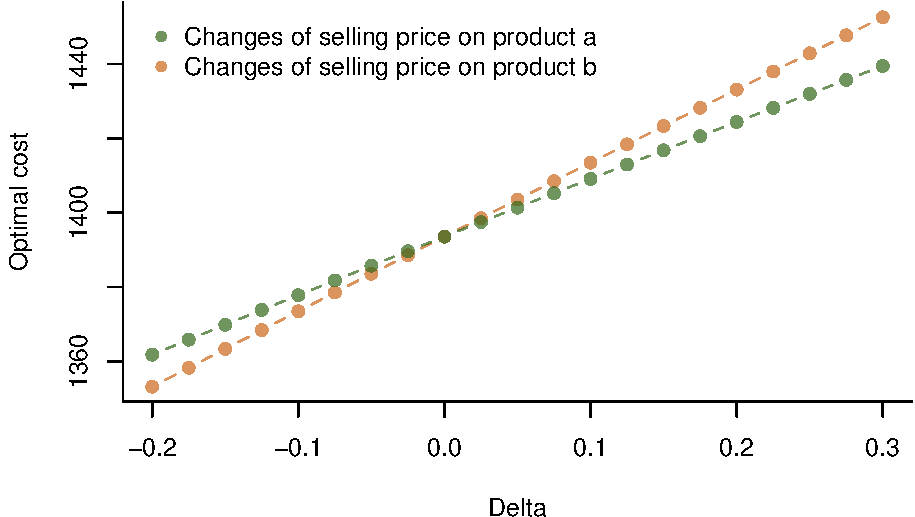
\includegraphics{Example-figure_files/figure-latex/demandunder-1.pdf}
\label{fig:demandunder}
\end{figure}

\section{Conclusion}
%\label{se:conclusion}

%%%%%%%%%%%%%%%%%%%%%%%%%%%%%%
\printbibliography
%%%%%%%%%%%%%%%%%%%%%%%%%%%%%%
\newpage
\begin{center}
{\bf\Large Appendices}
\end{center}

\appendix
\section{Sensitivity Report}
\label{se:report}

\begingroup\fontsize{7}{9}\selectfont
\begin{longtable}{cccccc}
\caption{Sensitivity Report: Variable Cells}
\label{tab:sen_var}\\
\toprule
variable & final value & reduced cost & coefficient & allowable increase & allowable decrease\\
\midrule
\endfirsthead
\multicolumn{6}{@{}l}{\textit{(continued)}}\\
\toprule
variable & final value & reduced cost & coefficient & allowable increase & allowable decrease\\
\midrule
\endhead
\
\endfoot
\bottomrule
\endlastfoot
$y_1^1$ & 7.1 & 0.0 & 5 & 6.0 & 3.8\\
$y_1^2$ & 0.0 & 5.0 & 5 & 10000.0 & 5.0\\
$y_1^3$ & 27.1 & 0.0 & 5 & 6.0 & 3.8\\
$y_1^4$ & 17.1 & 0.0 & 5 & 6.0 & 3.8\\
$y_1^5$ & 17.1 & 0.0 & 5 & 6.0 & 3.8\\
\addlinespace
$y_1^6$ & 0.0 & 5.0 & 5 & 10000.0 & 5.0\\
$y_1^7$ & 0.0 & 5.0 & 5 & 10000.0 & 5.0\\
$y_1^8$ & 0.0 & 5.0 & 5 & 10000.0 & 5.0\\
$y_1^9$ & 7.1 & 0.0 & 5 & 6.0 & 3.8\\
$y_1^{10}$ & 17.1 & 0.0 & 5 & 6.0 & 3.8\\
\addlinespace
$y_1^{11}$ & 0.0 & 5.0 & 5 & 10000.0 & 5.0\\
$y_1^{12}$ & 0.0 & 5.0 & 5 & 10000.0 & 5.0\\
$y_2^1$ & 0.0 & 7.0 & 7 & 10000.0 & 7.0\\
$y_2^2$ & 0.0 & 7.0 & 7 & 10000.0 & 7.0\\
$y_2^3$ & 10.0 & 0.0 & 7 & 2.7 & 4.3\\
\addlinespace
$y_2^4$ & 30.0 & 0.0 & 7 & 2.7 & 4.3\\
$y_2^5$ & 0.0 & 4.3 & 7 & 10000.0 & 4.3\\
$y_2^6$ & 0.0 & 7.0 & 7 & 10000.0 & 7.0\\
$y_2^7$ & 40.0 & 0.0 & 7 & 2.7 & 4.3\\
$y_2^8$ & 60.0 & 0.0 & 7 & 2.7 & 4.3\\
\addlinespace
$y_2^9$ & 30.0 & 0.0 & 7 & 2.7 & 4.3\\
$y_2^{10}$ & 0.0 & 7.0 & 7 & 10000.0 & 7.0\\
$y_2^{11}$ & 0.0 & 7.0 & 7 & 10000.0 & 7.0\\
$y_2^{12}$ & 0.0 & 7.0 & 7 & 10000.0 & 7.0\\
$z_1^1$ & 0.0 & 6.0 & 6 & 10000.0 & 6.0\\
\addlinespace
$z_1^2$ & 12.9 & 0.0 & 6 & 3.8 & 6.0\\
$z_1^3$ & 0.0 & 6.0 & 6 & 10000.0 & 6.0\\
$z_1^4$ & 0.0 & 6.0 & 6 & 10000.0 & 6.0\\
$z_1^5$ & 0.0 & 6.0 & 6 & 10000.0 & 6.0\\
$z_1^6$ & 2.9 & 0.0 & 6 & 3.8 & 6.0\\
\addlinespace
$z_1^7$ & 32.9 & 0.0 & 6 & 3.8 & 6.0\\
$z_1^8$ & 42.9 & 0.0 & 6 & 3.8 & 6.0\\
$z_1^9$ & 0.0 & 6.0 & 6 & 10000.0 & 6.0\\
$z_1^{10}$ & 0.0 & 6.0 & 6 & 10000.0 & 6.0\\
$z_1^{11}$ & 2.9 & 0.0 & 6 & 3.8 & 6.0\\
\addlinespace
$z_1^{12}$ & 32.9 & 0.0 & 6 & 3.8 & 6.0\\
$z_2^1$ & 40.0 & 0.0 & 6 & 4.3 & 2.7\\
$z_2^2$ & 20.0 & 0.0 & 6 & 4.3 & 2.7\\
$z_2^3$ & 0.0 & 6.0 & 6 & 10000.0 & 6.0\\
$z_2^4$ & 0.0 & 6.0 & 6 & 10000.0 & 6.0\\
\addlinespace
$z_2^5$ & 0.0 & 0.0 & 6 & 4.3 & 2.7\\
$z_2^6$ & 0.0 & 0.0 & 6 & 4.3 & 2.7\\
$z_2^7$ & 0.0 & 6.0 & 6 & 10000.0 & 6.0\\
$z_2^8$ & 0.0 & 6.0 & 6 & 10000.0 & 6.0\\
$z_2^9$ & 0.0 & 6.0 & 6 & 10000.0 & 6.0\\
\addlinespace
$z_2^{10}$ & 10.0 & 0.0 & 6 & 4.3 & 2.7\\
$z_2^{11}$ & 50.0 & 0.0 & 6 & 4.3 & 2.7\\
$z_2^{12}$ & 50.0 & 0.0 & 6 & 4.3 & 2.7\\
$x_1$ & 207.1 & 0.0 & 0 & 6.0 & 3.8\\
$x_2$ & 210.0 & 0.0 & 0 & 2.7 & 4.3\\*
\end{longtable}
\endgroup{}

\begingroup\fontsize{6}{9}\selectfont
\begin{longtable}{cccccc}
\caption{Sensitivity Report: Constraints}
\label{tab:sen_con}\\
\toprule
row & final value & shadow price & constraint RHS & allowable increase & allowable decrease\\
\midrule
\endfirsthead
\multicolumn{6}{@{}l}{\textit{(continued)}}\\
\toprule
row & final value & shadow price & constraint RHS & allowable increase & allowable decrease\\
\midrule
\endhead
\
\endfoot
\bottomrule
\endlastfoot
time\_A & 2088.6 & 0.0 & 2200 & 10000.0 & 111.4\\
time\_B & 2500.0 & -0.9 & 2500 & 20.0 & 50.0\\
time\_C & 3337.1 & 0.0 & 3500 & 10000.0 & 162.9\\
over\_1\textasciicircum{}1 & 200.0 & -5.0 & 200 & 7.1 & 10000.0\\
over\_1\textasciicircum{}2 & 207.1 & 0.0 & 220 & 10000.0 & 12.9\\
\addlinespace
over\_1\textasciicircum{}3 & 180.0 & -5.0 & 180 & 27.1 & 10000.0\\
over\_1\textasciicircum{}4 & 190.0 & -5.0 & 190 & 17.1 & 10000.0\\
over\_1\textasciicircum{}5 & 190.0 & -5.0 & 190 & 17.1 & 10000.0\\
over\_1\textasciicircum{}6 & 207.1 & 0.0 & 210 & 10000.0 & 2.9\\
over\_1\textasciicircum{}7 & 207.1 & 0.0 & 240 & 10000.0 & 32.9\\
\addlinespace
over\_1\textasciicircum{}8 & 207.1 & 0.0 & 250 & 10000.0 & 42.9\\
over\_1\textasciicircum{}9 & 200.0 & -5.0 & 200 & 7.1 & 10000.0\\
over\_1\textasciicircum{}10 & 190.0 & -5.0 & 190 & 17.1 & 10000.0\\
over\_1\textasciicircum{}11 & 207.1 & 0.0 & 210 & 10000.0 & 2.9\\
over\_1\textasciicircum{}12 & 207.1 & 0.0 & 240 & 10000.0 & 32.9\\
\addlinespace
under\_1\textasciicircum{}1 & 207.1 & 0.0 & 200 & 7.1 & 10000.0\\
under\_1\textasciicircum{}2 & 220.0 & 6.0 & 220 & 10000.0 & 12.9\\
under\_1\textasciicircum{}3 & 207.1 & 0.0 & 180 & 27.1 & 10000.0\\
under\_1\textasciicircum{}4 & 207.1 & 0.0 & 190 & 17.1 & 10000.0\\
under\_1\textasciicircum{}5 & 207.1 & 0.0 & 190 & 17.1 & 10000.0\\
\addlinespace
under\_1\textasciicircum{}6 & 210.0 & 6.0 & 210 & 10000.0 & 2.9\\
under\_1\textasciicircum{}7 & 240.0 & 6.0 & 240 & 10000.0 & 32.9\\
under\_1\textasciicircum{}8 & 250.0 & 6.0 & 250 & 10000.0 & 42.9\\
under\_1\textasciicircum{}9 & 207.1 & 0.0 & 200 & 7.1 & 10000.0\\
under\_1\textasciicircum{}10 & 207.1 & 0.0 & 190 & 17.1 & 10000.0\\
\addlinespace
under\_1\textasciicircum{}11 & 210.0 & 6.0 & 210 & 10000.0 & 2.9\\
under\_1\textasciicircum{}12 & 240.0 & 6.0 & 240 & 10000.0 & 32.9\\
over\_2\textasciicircum{}1 & 210.0 & 0.0 & 250 & 10000.0 & 40.0\\
over\_2\textasciicircum{}2 & 210.0 & 0.0 & 230 & 10000.0 & 20.0\\
over\_2\textasciicircum{}3 & 200.0 & -7.0 & 200 & 10.0 & 10000.0\\
\addlinespace
over\_2\textasciicircum{}4 & 180.0 & -7.0 & 180 & 30.0 & 10000.0\\
over\_2\textasciicircum{}5 & 210.0 & -2.7 & 210 & 0.0 & 4.0\\
over\_2\textasciicircum{}6 & 210.0 & 0.0 & 210 & 10000.0 & 0.0\\
over\_2\textasciicircum{}7 & 170.0 & -7.0 & 170 & 40.0 & 10000.0\\
over\_2\textasciicircum{}8 & 150.0 & -7.0 & 150 & 60.0 & 10000.0\\
\addlinespace
over\_2\textasciicircum{}9 & 180.0 & -7.0 & 180 & 30.0 & 10000.0\\
over\_2\textasciicircum{}10 & 210.0 & 0.0 & 220 & 10000.0 & 10.0\\
over\_2\textasciicircum{}11 & 210.0 & 0.0 & 260 & 10000.0 & 50.0\\
over\_2\textasciicircum{}12 & 210.0 & 0.0 & 260 & 10000.0 & 50.0\\
under\_2\textasciicircum{}1 & 250.0 & 6.0 & 250 & 10000.0 & 40.0\\
\addlinespace
under\_2\textasciicircum{}2 & 230.0 & 6.0 & 230 & 10000.0 & 20.0\\
under\_2\textasciicircum{}3 & 210.0 & 0.0 & 200 & 10.0 & 10000.0\\
under\_2\textasciicircum{}4 & 210.0 & 0.0 & 180 & 30.0 & 10000.0\\
under\_2\textasciicircum{}5 & 210.0 & 6.0 & 210 & 10000.0 & 0.0\\
under\_2\textasciicircum{}6 & 210.0 & 6.0 & 210 & 10000.0 & 0.0\\
\addlinespace
under\_2\textasciicircum{}7 & 210.0 & 0.0 & 170 & 40.0 & 10000.0\\
under\_2\textasciicircum{}8 & 210.0 & 0.0 & 150 & 60.0 & 10000.0\\
under\_2\textasciicircum{}9 & 210.0 & 0.0 & 180 & 30.0 & 10000.0\\
under\_2\textasciicircum{}10 & 220.0 & 6.0 & 220 & 10000.0 & 10.0\\
under\_2\textasciicircum{}11 & 260.0 & 6.0 & 260 & 10000.0 & 50.0\\
\addlinespace
under\_2\textasciicircum{}12 & 260.0 & 6.0 & 260 & 10000.0 & 50.0\\*
\end{longtable}
\endgroup{}

\section{Costs on boundaries}
\label{se:costfun}

\begin{figure}[ht]
\centering
\caption{Costs on boundary 1}
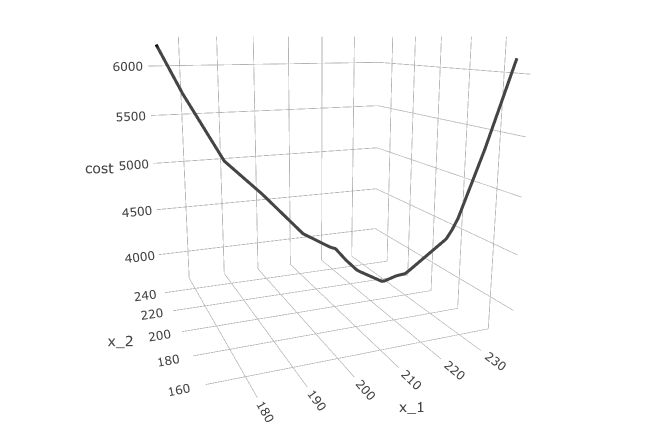
\includegraphics[width=\textwidth]{Example-figure_files/figure-latex/boundary1.png}
\label{fig:bd1}
\end{figure}

\begin{figure}[ht]
\centering
\caption{Costs on boundary 2}
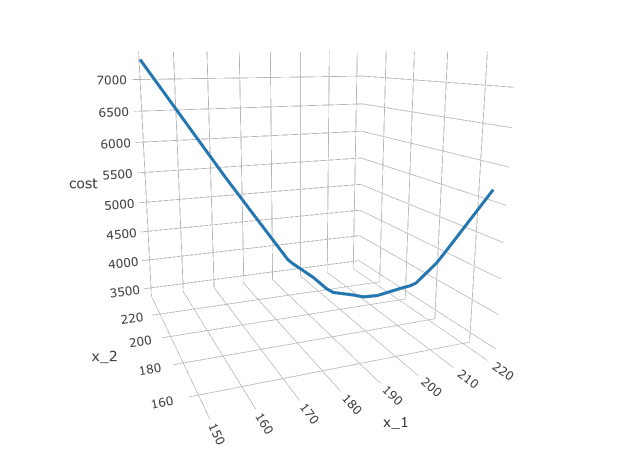
\includegraphics[width=\textwidth]{Example-figure_files/figure-latex/boundary2.png}
\label{fig:bd2}
\end{figure}


\end{document}
